\documentclass{article}
\usepackage{tikz}
\usetikzlibrary{calc, positioning}

\begin{document}

\begin{figure}[h]
    \centering
    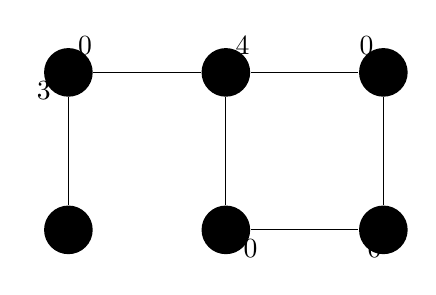
\begin{tikzpicture}[node distance = 1cm, auto]
        % Define nodes
        \node[circle, fill=black] (v0) at (0,0) {0};
        \node[circle, fill=black] (v1) at (2,0) {4};
        \node[circle, fill=black] (v2) at (4,0) {0};
        \node[circle, fill=black] (v3) at (0,-2) {3};
        \node[circle, fill=black] (v4) at (2,-2) {0};
        \node[circle, fill=black] (v5) at (4,-2) {0};

        % Draw edges
        \draw (v0) -- (v1);
        \draw (v1) -- (v2);
        \draw (v0) -- (v3);
        \draw (v1) -- (v4);
        \draw (v2) -- (v5);
        \draw (v4) -- (v5);

        % Position labels
        \path let \p1=($(v0)-(v1)$), \n1={atan2(\y1,\x1)} in node [above right] at ($(v0)+(\n1-90:.1)$) {0};
        \path let \p1=($(v1)-(v2)$), \n1={atan2(\y1,\x1)} in node [above right] at ($(v1)+(\n1-90:.1)$) {4};
        \path let \p1=($(v2)-(v1)$), \n1={atan2(\y1,\x1)} in node [above left] at ($(v2)+(\n1+90:.1)$) {0};
        \path let \p1=($(v0)-(v3)$), \n1={atan2(\y1,\x1)} in node [below left] at ($(v0)+(\n1+90:.1)$) {3};
        \path let \p1=($(v4)-(v1)$), \n1={atan2(\y1,\x1)} in node [below right] at ($(v4)+(\n1+90:.1)$) {0};
        \path let \p1=($(v5)-(v2)$), \n1={atan2(\y1,\x1)} in node [below left] at ($(v5)+(\n1+90:.1)$) {0};
    \end{tikzpicture}
    \caption{Graph of Proposition \protect\ref{cota2}}
    \label{fig:graph}
\end{figure}

{\protect\small The condition {$g(\Gamma)\geq 5$} is necessary in Proposition \protect\ref{cota2}.}

\end{document}